

% Overview Illustration
\begin {figure*}%[!hbtp]
\centering
\begin{tikzpicture}[node distance=2.5cm]

\node (interpreter) [component] {Code Interpreter};
\node (composer) [component, right of=interpreter, xshift=3cm] {Graph Composer};
\node (detector) [component, right of=composer, xshift=3cm] {Code Smells \\ Detector};

\node (astroid) [library, above of=interpreter] {Astroid};
\node (mongodb) [database, below of=interpreter, xshift=2.5cm] {Mongo DB};
\node (kg) [database, below of=composer, xshift=2.5cm] {Neo4j};

\node (driver) [driver, left of=interpreter, xshift=-0.6cm] {Driver};
\node (result) [driver, above of=detector, yshift=-1cm] {Result};


% Arrows
\path (interpreter) edge[arrow, bend left] node[on arrow, anchor=east, xshift=0.4cm] {Entire codebase} (astroid);
\path (astroid) edge[arrow, bend left] node[on arrow, anchor=west, xshift=-0.4cm] {Abstract Syntax Trees \\ \& Inferences} (interpreter);
\path (interpreter) edge[arrow, bend right] node[on arrow, anchor=east, xshift=0.7cm] {Insertion of JSON documents of \\ entities and relationships in mixture} (mongodb);
\path (mongodb) edge[arrow, bend left] node[on arrow, yshift=-0.3cm] {Retrieval of JSON documents of \\ entities and relationships in order} (composer);
\path (composer) edge[arrow, bend right] node[on arrow, yshift=0.1cm] {Creation queries of \\ Entities and Relationships} (kg);
\path (detector) edge[arrow, bend right] node[on arrow, yshift=0.1cm] {Code smells pattern queries} (kg);
\path (kg) edge[arrow, bend right] node[on arrow, yshift=0.1cm] {Matching entities and relationships} (detector);


\path (driver) edge[flow] (interpreter);
\path (interpreter) edge[flow] (composer);
\path (composer) edge[flow] (detector);
\path (detector) edge[flow] (result);



\end{tikzpicture}
\caption{Overview of CSKG system}
\label{fig:cskg-overview}
\end{figure*}



\section{Implementation}
\label{sec:imple}

This section describes the implementation of the CSKG (Code Smells - Knowledge Graph) system. An overview of the system is shown in \autoref{fig:cskg-overview}. 

The system is composed by three major components, which are: Code Interpreter, Graph Composer and Code Smells Detector. All the three components are driven by the Driver component. It employs a list of external libraries and tools, as detailed in \autoref{sec:appendix-a}. It utilizes MongoDB for the storage of intermediate data and Neo4j as the database for the knowledge graph. The Astroid library is leveraged to extract the abstract syntax tree, and the entire system is developed in Python.

In support of transparency and reproducibility, the source code and data associated with this work is available on GitHub\footnote{\url{https://github.com/cloudyyoung/cskg}}.


\subsubsection{Code Interpreter}

The process begins by loading all Python files from the target codebase and extracting their AST trees using the Astroid library. Each AST tree is then recursively and thoroughly examined to identify and extract significant entities and relationships. When an entity or relationship of interest (as specified in \autoref{tab:ents-and-rels}) is found, the component compiles and yields this information along with the necessary property data.

The \texttt{Driver} component interacts with MongoDB database to store these entities and relationships. It organizes them into separate collections, allowing for structured and sequential data retrieval. This setup facilitates the \texttt{GraphComposer}'s task of reading the data in an ordered manner, prioritizing entities first and then relationships.

% To address the issue of functions and classes having identical names within different scopes, the system not only uses a \texttt{name} property but also a \texttt{qualified\_name} property. The \texttt{qualified\_name} is akin to a full address, detailing where in the code hierarchy an entity resides. It includes the namespace and parent structures, ensuring each identifier is uniquely identified regardless of similar names in other scopes. 



\subsubsection{Graph Composer}

Following the initial steps, this component begins constructing the knowledge graph. It starts by integrating all the identified entities and then incorporates the relationships. This construction involves populating Neo4j database using Cypher queries for efficient data entry and connection. \autoref{fig:schema-vis} provides a detailed representation of the knowledge graph's relational dynamics and structural organization, visually illustrating the connections and relationships between nodes.

In Neo4j database, relationships can only be established if the relevant entities already exist. Therefore, to correctly set up the knowledge graph, it's essential to first insert all entities into the database before adding relationships. This step-by-step approach utilizing Mongo DB ensures that relationships are correctly linked to the pre-existing entities, preserving the graph's structural integrity and coherence.



\begin{figure}[htbp]
\begin{center}
    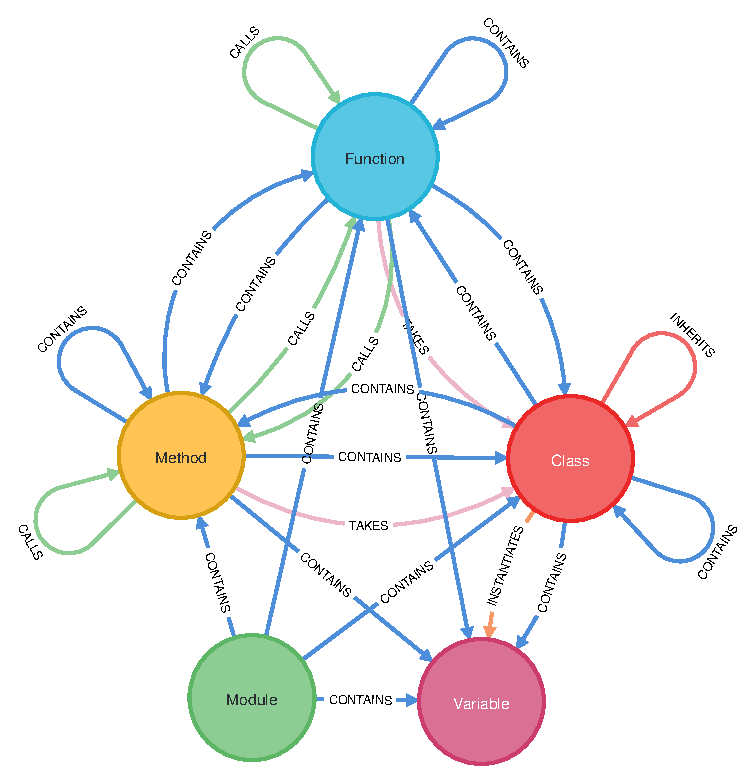
\includegraphics[width=0.4\textwidth]{figures/graph.eps}
\end{center}
\caption{Neo4j Scheme Visualization (To be updated*)}
\label{fig:schema-vis}
\end{figure}


\subsubsection{Code Smells Detector}
...

\newpage
\newpage
\newpage
\newpage
